\section{Quantenhardware}
\label{sec:quantenhardware}

Die Realisierung eines Quantencomputers ist durch hohe technische Herausforderungen geprägt. Um die besonderen Eigenschaften der Qubits eines Quantencomputers, wie Superposition und Verschränkung, nutzen zu können, müssen sie durch externe Einflüsse geschützt werden und die Dekoheränz minimiert werden.
Äußere Einflüsse wie Temperaturschwankungen, elektromagnetische Felder oder Strahlung aller Art können die Qubits beeinflussen. Aus diesem Grund werden Quantencomputer bei extrem niedrigen Temperaturen und in einem Vakuum betrieben.\\

Außerdem ist nicht nur die Herstellung der Qubits eine Herausforderung, sondern auch die Steuerung, Auslesung und Korrektheit von physikalischen Qubits.

\subsection{Dekohärenz}
\label{sub:dekohaerenz}
Dekoheränz ist ein zentrales Konzept, welches wichtig in der Entwicklung von Quantencomputern ist. Der Prozess der Dekoheränz beschreibt den Verlust der koheränten Quanteneigentschaften eines Qubits durch Wechselwirkung mit der Umgebung.
Diese Veränderung führt zu einem Übergang von quantenmechanischem Verhalten zu einem klassischem Verhalten von Bits.\footnote{\cite{breuer_decoherence_2007}}\\

In der Quantenmechanik können Systeme in Überlagerungszuständen existieren, wobei mehrere Zustände gleichzeitig eingenommen werden können. Diese Eigenschaft erklärt auch das Phänomen der Quanteninterferenz.
Äußere Einflüsse durch die Umgebung kann eine Verschränkung von Qubits zerstören. Dies führt dazu, dass die Phasenbeziehungen zwischen den Qubits beeinflusst oder gar aufgehoben werden.
Folgernd verliert das System die Interferenzeffekte und verhält sich zunehmend klassischer. Diese Zeit nennt man Dekoheränzzeit.\\

Die \textbf{Dekoheränzzeit} ($T_2$) eines Qubits misst die Länge der Zeit, in der es in der Lage bleibt kohärent zu bleiben, welcher danach von äußeren Einflüssen zerstört wird\footnote{\cite{bacciagaluppi_role_2020}}.
Neben $T_2$ wird auch häufig die \textbf{Relaxationszeit} ($T_1$) gemessen, welche angibt, wie lange ein Qubit im angeregten Zustand bleibt, bevor es auf sein Grundzustand zurückfällt.
In der Realität ist die Dekoheränzzeit jedoch in den meisten Fällen kürzer als die Relaxationszeit.\\

\textbf{Berechnung der Dekoheränzzeit}\\
Durch eine Messung der zeitlichen Abnahme der Koheränz eines beispielhaften Qubits kann die Dekoheränzzeit eines Systems festgelegt werden.
Bei einem Quantencomputer, der auf dem Spin eines Teilchen beruht, kann dies durch die \textbf{Spin-Echo-Methode} gemessen werden.
Quantencomputer, die auf anderen Qubits basieren, haben equivalente Methoden um die Kohärenz zu messen.\\

Das einfachste Modell zur Beschreibung der Dekoheränzzeit ist die \textbf{Exponentielle Abnahme der Kohärenz}

\begin{equation}
    C(t) = C(0)*e^{-t/T_2}
\end{equation}

Dabei ist:\\
$C(t)$ Die Kohärenz des Qubits zum Zeitpunkt t\\
$C(0)$ Die initiale Koheränz\\
$T_2$ Die Dekoheränzzeit\\

Indem man den Kohärenzverlust experimentell misst und die Werte in eine exponentielle Abklingfunktion einpasst, erhält man $T_2$.\\

\begin{tcolorbox}[title=Kommentar,
    title filled=false,
    colback=cyan!5!white,
    colframe=cyan!75!black]
    Die \textbf{Dekoheränzzeit} kann auch durch genauere, jedoch auch deutlich kompliziertere Weise errechnet werden.
    Bekannte Methoden hierfür wären zum Beispiel die Spektrale Analyse, Dynamische Entkopplung, Hahn-Echo und Ramsey-Interferometrie.
    Außerdem wird duch das häufige messen der Dekoheränzzeit diese indirekt verlängert. Diesen Effekt nennt man Quanten-Zeno-Effekt.\\
    Zuletzt muss auch die Lindblad-Gleichung\footnote{\cite{bacciagaluppi_role_2020}} genannt werden, welche den Zeitverlauf der Dichtematrix in einem Offenen Quantensystem beschreibt.
    \begin{equation}
        \frac{dp}{dt} = -i[H,p]+\sum_i(L_ipL^\dagger_i-\frac{1}{2}\{L^\dagger_i L_i,p\})
    \end{equation}
    Diese Themen sprengen jedoch den Rahmen dieser Arbeit in Richtung Physik und werden deswegen nicht weiter behandelt.
\end{tcolorbox}

\subsection{Universelle Quantencomputer}
\label{sub:universelle_quantencomputer}
Universelle Quantencomputer beruhen grundlegend auf einem Gatter Modell, wie bereits in diesem Artikel beschrieben. Im Folgenden werden drei der meist erforschten
Methoden, welche dieses Modell physikalisch umsetzen, beschrieben.\\

Ein prominentes Beispiel für die Umsetzung eines universellen Quantencomputers ist der \textbf{Sycamore Chip}\footnote{\cite{arute_quantum_2019}}, welcher auf supraleitenden Qubits basiert.
Dieser Chip ist in einem Gatter angeordnet für die Kommunikation zwischen Qubits und die Durchführung von Quantenoperationen.\\

\begin{figure}[H]
    \centering
    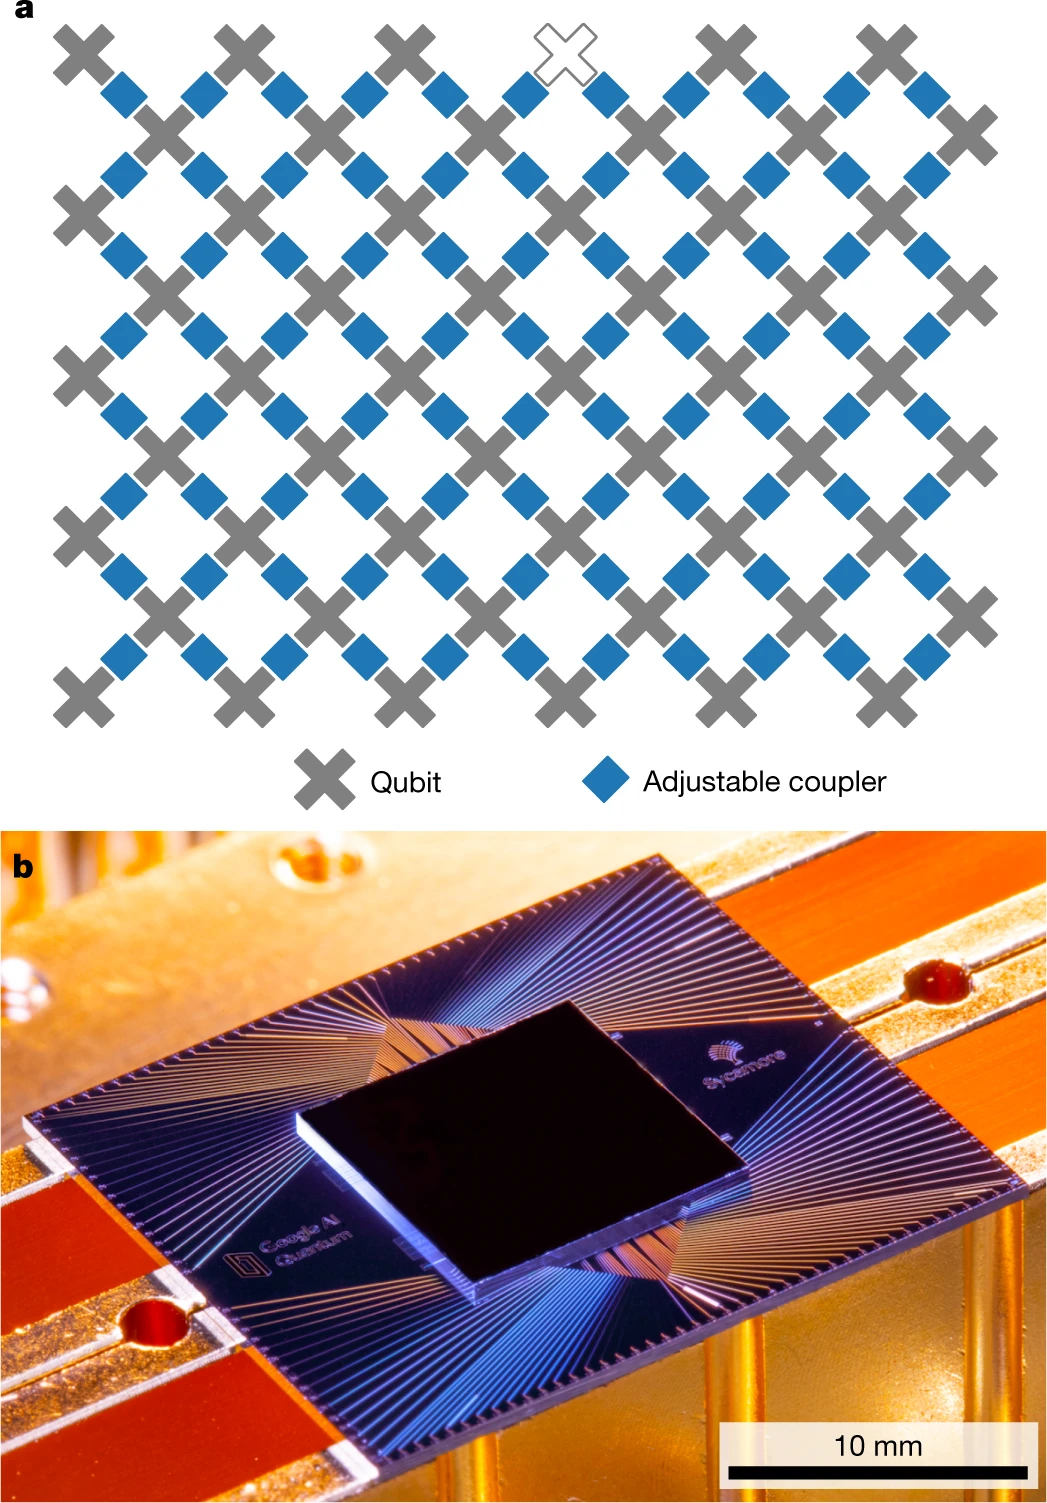
\includegraphics[width=0.7\linewidth]{img/SycamoreChip.png}
    \caption{Sycamore Chip von Google \cite{arute_quantum_2019}}
    \label{fig:Sycamore}
\end{figure}

\subsubsection{Supraleitende Qubits}
\label{subsub:superleiter}
Quantencomputer mit Supraleitern funktionieren mit elektrischen Schaltkreisen, die bei Temperaturen nahe dem absoluten Nullpunkt betrieben werden. Solche Temperaturen sind nötig,
um die supraleitende Eigenschaft aufrecht zu erhalten.\\

Zwei häufig benutzte Qubit-Typen dieser elektrischen Schaltkreise sind:\\
\textbf{Transmon-Qubits}, basieren auf der Ladung des Energieniveaus, welche durch eine Josephson-Junktion kontrolliert werden.\\
\textbf{Flux-Qubits} werden auch durch Josephson-Junktions kontrolliert, beruhen jedoch auf dem magnetischen Fluss in der Schleife.\\

Beide Ansätze basieren auf dem \textbf{Josephson-Effekt}\footnote{\cite{kjaergaard_superconducting_2020}}, welcher auftritt, wenn ein supraleitender Strom durch eine dünne Isolierschicht zwischen zwei Supraleitern fließt.\\
Dieser Effekt hat zur Folge, dass eine nichtlineare Energie für die Phasenunterscheidung der Qubits genutzt wird.\\

\begin{figure}[H]
    \centering
    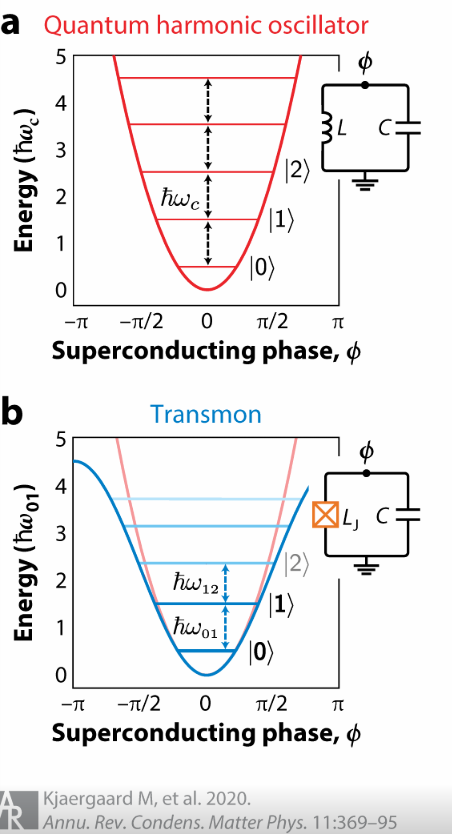
\includegraphics[width=0.75\linewidth]{img/JJ.png}
    \caption{Josephson-Effekt mit einer Josephson Junktion \cite{kjaergaard_superconducting_2020}}
    \label{fig:Josephson-junktion}
\end{figure}

In der vorliegenden Abbildung wird der Unterschied zwischen einer harmonischen Quantenschwankung (a) und der nichtlinearen Schwankung des Energieniveau der Josephson Junktion (b) abgebildet.\\

Der Phasenunterschied bei der harmonischen Oscellation, gekennzeichnet als $\hbar\omega_c$, ist identisch. Auf der Abbildung ist zu sehen, dass das Energieniveau der Phasen zwischen $\ket{0} \leftrightarrow \ket{1}$
und $\ket{1} \leftrightarrow \ket{2}$ identisch ist und dadurch nicht unterschieden werden kann zwischen welcher Phase gewechselt wurde.\\

Mit einer Josephson Junktion kann jedoch eine nichtlineare Schwankung des Energieniveaus erreicht werden, die auf der Abbildung als orangenes $\boxtimes$ gekennzeichnet ist (b).
Durch diese nichtlineare Schwankung ist das Energieniveau zwischen den Phasen $\ket{0} \leftrightarrow \ket{1}$ und $\ket{1} \leftrightarrow \ket{2}$ unterschiedlich groß und kann somit unterschieden werden.
Der als $\hbar\omega_{01}$ gekennzeichnete Energieunterschied ist unser Qubit.\\

\textbf{Steuerung und Auslesung}\\
Die Steuerung der Josephson-Junktion erfolgt durch Mikrowellenpulse, welche die Energie des Qubits verändern. Die Auslesung erfolgt durch eine Mikrowellenresonanz um die Energie des Qubits zu messen.\\

\subsubsection{Quantenpunkte}
\label{subsub:quantenpunkte}
Quantencomputer basierend auf Quantenpunkten, auch Quantum-Dot\footnote{\cite{loss_quantum_1998}} genannt, nutzen winzige Halbleiterstrukturen um Qubits zu realisieren.
Quantum-Dots sind künstlich erzeugte Nano-Partikel, in denen Elektronen in drei Dimensionen eingeschlossen sind, was zu quantisierten Energiezuständen führt.\\

Die Größe eines Quantum-Dots ist typischerweise 2-10 Nanometer und es schließt eine kleine Anzahl oder ein einzelnes Elektron ein.
Für die Fertigung werden oftmals Galliumarsenid (GaAs) oder Silizium (Si) verwendet. Der physikalische Einschluss der Elektronen schränkt ihre
Bewegung stark ein, wodurch ein quantisiertes Energieniveau entsteht. Dies ähnelt dem Energieniveaus eines Atoms, weswegen Quantum-Dots auch als künstliche Atome bezeichnet werden.\\

Die Zustände der Qubits werden durch die Eigenschaften einzelner Elektronen in den Quantum Dots definiert. Es gibt zwei Hauptansätze zur Realisierung von Qubits mit Quantum Dots.\\

\textbf{Ladungs-Qubits}\\
Der Ladungszustand eines Quantum Dots kann als Qubit verwendet werden. Die Ladung eines Elektrons kann entweder 0 oder 1 sein, was als $\ket{0}$ und $\ket{1}$ interpretiert wird.
Für eine Messung wird der Ladungszustand mit einer Kapazitätsmessung der Tunnelströme ermittelt.
Für die Manipulation des Qubits werden elektrische Felder verwendet, um die Elektronen in den Quantum Dots zu bewegen.\\

Diese Methode ist durch die Ladungsquantisierung sehr genau, jedoch auch sehr empfindlich gegenüber Störungen durch die Umgebung.\\

\textbf{Spin-Qubits}\\
Die Spin-Eigenschaften von Elektronen in Quantum Dots können auch als Qubit verwendet werden. Hierbei sind die beiden Spinrichtungen($\uparrow$ für Spin-Up und $\downarrow$ für Spin-Down).
Diese beiden Spinrichtungen entsprechen den Zuständen $\ket{0}$ und $\ket{1}$ und die Kombination aus beiden Zuständen ergibt eine Superposition.\\

\begin{figure}[H]
    \centering
    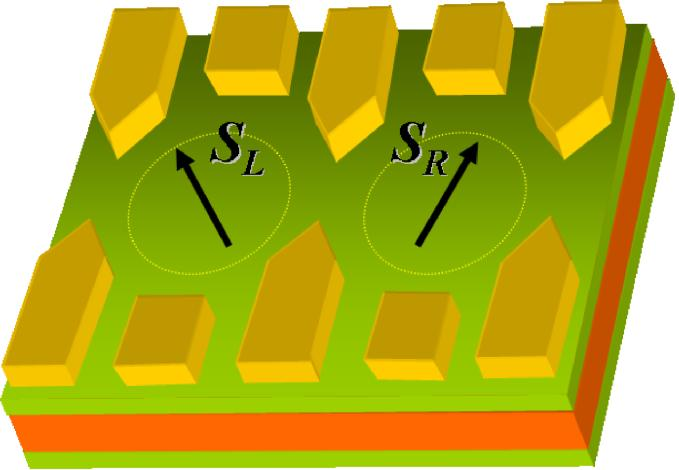
\includegraphics[width=0.75\linewidth]{img/QD.png}
    \caption{Ein doppel Quantum-Dot Qubit \cite{Golovach_condensed_2006}}
    \label{fig:double-Quantum-Dot}
\end{figure}

In der Abbildung ist ein Doppel Quantum-Dot Qubit dargestellt. Sowohl in $S_L$ als auch $S_R$ befinden sich Elektornen. Beide können separat voneinander, sowohl im Spin als auch in der Ladung, manipuliert werden.
Durch die physikalische Nähe der beiden Quantum-Dots können durch Tunnelkopplung und Austauschwechselwirkung die beiden Qubits miteinander verschränkt werden.\\

Die Umsetzung dieser Methode beschränkt sich hauptsächlich auf die Spin-Variante. Der Grund dafür ist, dass durch die hohe Ladungsanforderung der Ladungsvariante die Qubits sehr empfindlich gegenüber Störungen sind.
Außerdem sind die Nachteile der Spin-Variante gegenüber der Ladungsvariante nicht so gravierend.\\
Jedoch sind die größten Herausforderungen die Herstellung der Halbleiterstrukturen und die Kontrolle der Elektronen in den Quantum-Dots.
Damit ist der größte Vorteil, die hohe Skalierbarkeit, auch der größte Nachteil, da die Herstellung und Kontrolle von vielen Quantum-Dots sehr aufwendig und schwierig ist.\\

\subsubsection{Topologische Quantencomputer}
\label{subsub:topologische_quantencomputer}
Der Ansatz von topologischen Quantencomputern\footnote{\cite{nayak_non-abelian_2008}} ist völlig anders als die bisher genannten. Im Gegensatz zu vorher erläuterten Quantencomputern, welche auf Eigenschaften einzelner Elektronen oder Energieniveaus basieren, basieren topologische Quantencomputer auf topologischen Eigenschaften von Materie.\\
Diese Methode soll das Problem der Dekoheränz minimieren, indem sie Qubits aus Majorana-Partikeln aufbauen.\\

\textbf{Topologie in der Physik}\\
In einem physikalischem System beschreibt die Topologie die Eigenschaften, welche sich nicht durch Deformation verändern lassen.
Ein Beispiel hierfür ist ein Kaffeebecher, der sich durch Verformung in eine Donutform umwandeln lässt. Beide haben die topologische Eigenschaft eines Loches.
Daraus folgernd ist es nicht möglich, einen Kaffeebecher oder ein Donut in eine Kugel zu verformen ohne die topologische Eigenschaft zu verändern.\\

\textbf{Funktionsweise}\\
Die physikalische Grundlage für topologische Quantencomputer liegt in speziellen Materialien und Systemen, die topologische Materiephasen unterstützen.
Ein prominentes Beispiel ist die Verwendung von Majorana-Quasiteilchen, die in bestimmten Supraleitern auftreten können.\\

\begin{figure}[H]
    \centering
    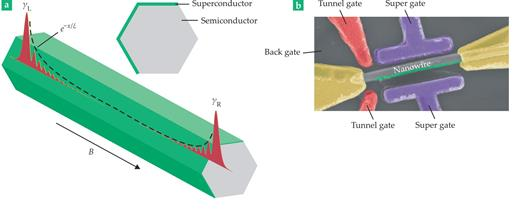
\includegraphics[width=0.75\linewidth]{img/Majorana.png}
    \caption{Nanowire mit Majorana-Quasiteilchen \cite{aguado_majorana_2020}}
    \label{fig:Majorana}
\end{figure}

In der Abbildung ist ein Nanowire dargestellt, der durch einen Supraleiter und ein Magnetfeld in eine topologische Phase gebracht wird.
Diese Art von Partikeln treten immer als Paar auf und bilden eine Art Brücke zwischen den Enden des Nanowire und besteht auf einer Vielzahl von Elektronen.
Diese Brücke wird durch die topologischen Eigenschaften der Majorana-Partikel stabilisiert und ist somit weniger anfällig gegenüber Störungen.\\


\begin{tcolorbox}[title=Kommentar,
    title filled=false,
    colback=cyan!5!white,
    colframe=cyan!75!black]
    Die Vertiefung, die durch den Quanten-Hall Effekt entsteht, wird nur oberflächlich behandelt. Sie ist jedoch essentiell für die Funktionsweise von Topologischen Quantencomputern.
\end{tcolorbox}

\textbf{Verflechtung}\\
Braiding ist der Prozess, bei dem die Majorana-Partikel miteinander verflochten werden, um die Quantenbits zu manipulieren. 
Dies passiert auf einer zweidimensionalen Oberfläche, auf der die Majorana-Partikel miteinander verflochten werden.\\

\begin{figure}[H]
    \centering
    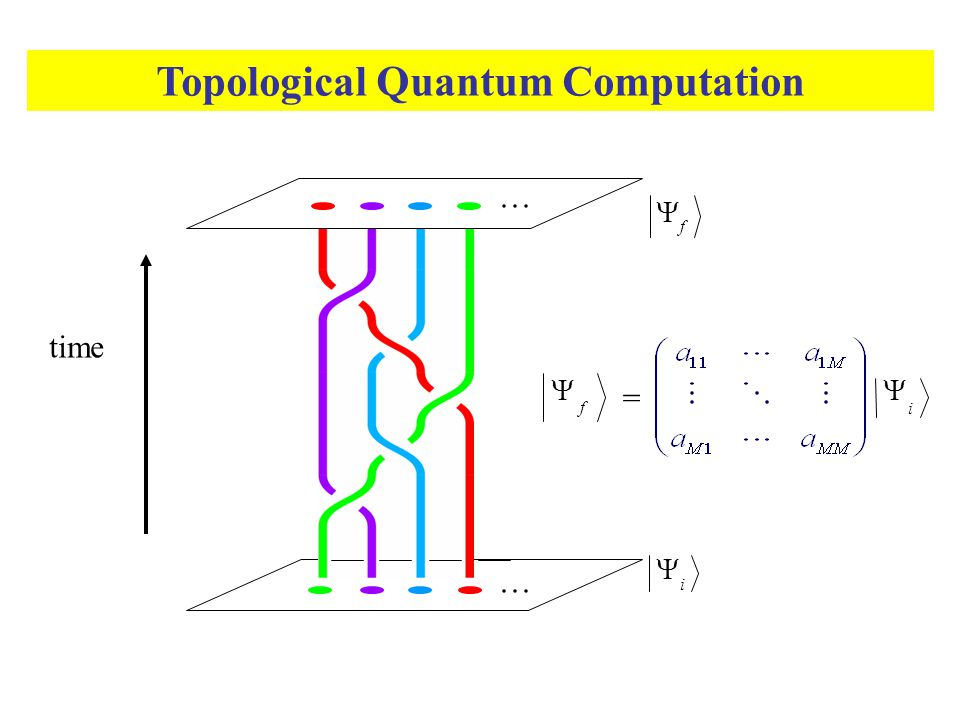
\includegraphics[width=0.75\linewidth]{img/TQC.png}
    \caption{Braiding von Majorana-Quasiteilchen}
    \label{fig:Braiding}
\end{figure}

Hierbei ist die Reihenfolge sehr wichtig, da durch diese Reihenfolge Quantenoperationen realisiert werden.
Jede Verflechtung entspricht einer Quantenoperation und durch die Kombination von mehreren Verflechtungen können beliebige Quantenoperationen realisiert werden.\\

Da die Informationen und Quantenoperationen in der Topologie steckt, sind sie gegenüber kleinen Fehlern in der Bewegung/Störungen unempfindlich.\\

\begin{tcolorbox}[title=Kommentar,
    title filled=false,
    colback=cyan!5!white,
    colframe=cyan!75!black]
    Die Technische Umsetzung von topologischen Quantencomputern ist deutlich komplizierter als es in diesem Abschnitt oberflächlich beschrieben ist.\\
    Bisher hat nur Google einen topologischen Quantencomputer vorgestellt, der jedoch noch nicht in der Lage ist, Quantenoperationen durchzuführen.
\end{tcolorbox}

\subsection{Quantum Error Correction}
\label{sub:quantum_error_correction}
Quantum Error Correction, oder auch QEC\footnote{\cite{qutech_academy_quantum_2018}} genannt, ist grundlegend wichtig für die funktionellen Betrieb eines Quantencomputers. Wie bereits in den vorherigen Abschnitten beschrieben,
sind Qubits sehr anfällig gegenüber Dekoheränz und Quantenrauschen.\\

\textbf{Warum ist Fehlerkorrektur notwendig}\\
Es ist unabdingbar, dass eine Fehlerkorrektur in Quantencomputern implementiert wird, da die Fehleranfälligkeit von physischen Qubits durch bessere Herstellung nur einen gewissen Grad an Fehlertoleranz aufbringen kann, welche nicht genug ist.\\

Fehler treten in Quantencomputer durch drei Hauptquellen auf.\\
1. \textbf{Dekoheränz:} Äußere Einflüsse wie Temperaturschwankungen oder elektromagnetische Felder zerstören die koheränten Eigenschaften der Qubits.\\
2. \textbf{Phasen-Flip-Fehler:} Die Phasenwinkel zwischen den Quantenzuständen werden verändert($\ket{0}\rightarrow\ket{0},\ket{1}\rightarrow-\ket{1}$).\\ 
3. \textbf{Bit-Flip-Fehler:} Die Zustände der Qubits werden verändert ($\ket{0}\rightarrow\ket{1},\ket{1}\rightarrow\ket{0}$).\\

Bei der Fehlerkorrektur von Quantencomputern ist jedoch zu beachten, dass diese nicht wie bei herkömmlichen Computern implementierbar ist, da durch das No-Cloning-Theorem keine Quanteninformationen kopiert werden können.\\

\textbf{Grundprinzip}\\
Quanten-Fehlerkorrektur verwendet \textbf{Redundanz} um Fehler zu detektieren und zu korrigieren, ohne dass die eigentliche Quanteninformationen direkt ausgelesen werden müssen.\\

Eine Art der Redundanz ist der Steane-Code, welcher auf 7 Qubits basiert. Dieser Zusammenschluss aus 7 Physischen Qubits bildet ein logisches Qubit,
welches maximal einen Fehler auf einem der 7 Qubits korrigieren kann. Treten jedoch mehrere Fehler auf, kann der Steane-Code diese nicht mehr korrigieren.\\

\begin{figure}[H]
    \centering
    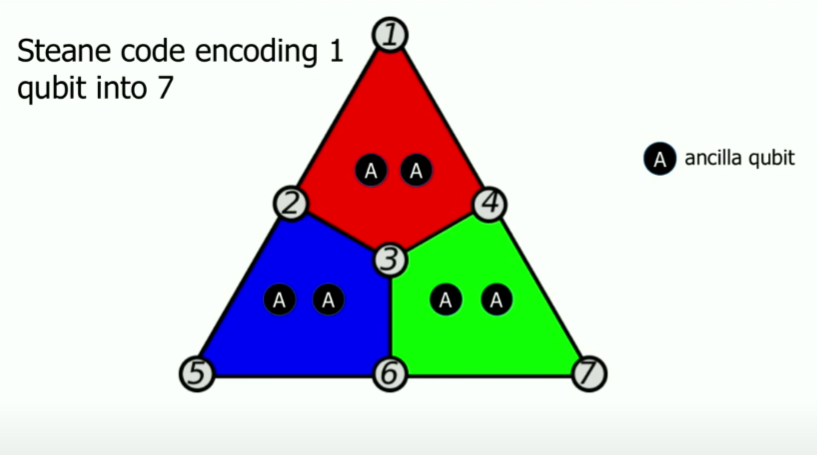
\includegraphics[width=0.75\linewidth]{img/Steane.png}
    \caption{Steane-Code \cite[2m30s]{qutech_academy_quantum_2018}}
    \label{fig:Steane}
\end{figure}

Um die Qubits zu überwachen werden zusätzliche Qubits benötigt. Der Grund hierfür ist die Daten-Qubits, in der Abbildung mit 1-7 gekennzeichnet, nicht direkt zu messen und den Quantenzustand zu bewahren.
Diese zusätzlichen Qubits werden als \textbf{Ancilla Qubit} bezeichnet und mit den eigentlichen Qubits verschränkt.\\

\textbf{Fehlertoleranz}\\
Diese Herangehensweise ist jedoch auch nicht perfekt. Die Ancilla Qubits sind gleichermaßen anfällig gegenüber Fehlern wie die eigentlichen Qubits.\\

\begin{figure}[H]
    \centering
    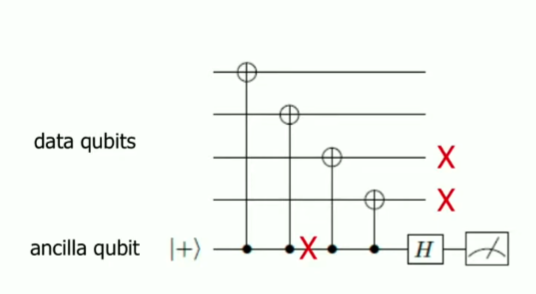
\includegraphics[width=0.75\linewidth]{img/Fehlertoleranz.png}
    \caption{Fehlertoleranz von Ancilla Qubits \cite[50s]{qutech_academy_quantum_2018}}
    \label{fig:Fehlertoleranz}
\end{figure}

Dieses Abbildung zeigt, wie ein einzelner Fehler in einem CNOT Gatter auf dem Ancilla Qubit Messung ein Daten-Qubits als fehlerhaft kennzeichnet und eigentlich richtige Daten-Qubits korrigiert.\\
Die Folge hieraus ist, dass die Fehlerkorrektur mit wenigen Qubits nicht ausreicht, um diesen logischen Qubit vollkommen fehlerfrei zu halten.\\

Hierbei werden zwischen zwei Paritätchecks unterschieden. Eine $Z$ und $X$ Parität, welche festlegen, ob der Fehler im CNOT Gatter des Ancilla Qubits oder in den Daten Qubits aufgetreten ist.\\

\textbf{Suface Code}\\
Eine weitere Methode zur Fehlerkorrektur ist der Surface Code, welcher auf einem 2D Gitter von Qubits basiert.
Dieser Code ist in der Lage Fehler zu detektieren und zu korrigieren, solange die Fehlerdichte unter einem bestimmten Wert bleibt.\\

Die Größe des Surface Codes ist variabel und kann skaliert werden, um die Fehlerkorrektur zu verbessern.
Es gibt jedoch ein Threshold, an der die Vergrößerung des Codes keine Verbesserung mehr bringt.
Durch die vorher besprochene Fehlertoleranz der Ancilla Qubits wird die Effektivität des Surface Codes gedeckelt.
Die Fehler in der Korrektur werden hierbei mehr, als wenn keine Korrektur vorgenommen wird und es würde keinen Sinn ergeben, den Surface Code weiter zu vergößern.\\

Die nachfolgende Abbildung eines Surface Codes des Grades $d=3$ zeigt wie die Qubits in einem 2D Gitter angeordnet sind und wie die Fehlerkorrektur durchgeführt wird.
Jede Überschneidung des Gatters stellt ein physisches Qubit dar. Die Kreise in den Quadraten sind die Ancilla Qubits, welche die Fehlerkorrektur durchführen.\\

\begin{figure}[H]
    \centering
    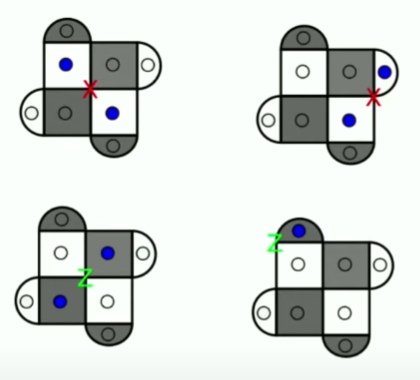
\includegraphics[width=0.6\linewidth]{img/Errors.png}
    \caption{Fehlerkorrektur durch Surface Code des Grades $d=3$ \cite[5m]{qutech_academy_quantum_2018}}
    \label{fig:Surface-Code}
\end{figure}

Ancilla Qubits in einem weißen Feld prüfen die Qubits auf ein logisches $X$ und Ancilla Qubits in einem Schwarzen Feld prüfen die Qubits auf ein logisches $Z$.\\

Ancilla Qubits, die einen Fehler erkennen, werden als Blau markiert. Durch die Position dieser und für welche Daten Qubits diese zuständig sind, wissen wir welche Qubits fehlerhaft sind.\\

\textbf{Praktische Umsetzung}\\
Am 09.12.2024 hat Google den ersten selbst korrigierenden Quantencomputer vorgestellt, der auf dem Surface Code basiert.
Der Chip namens \textbf{Willow}\footnote{\cite{acharya_quantum_2024}} basiert auf 105 physischen Qubits, wobei diese auf der 7x7 Surface Code Architektur aufbaut.
Dies resultiert in 49 Qubits, die deutlich weniger anfällig gegen Fehler sind als phyische Qubits. Die restlichen Qubits werden für Parität und Error Korrektur gebraucht.\\

\begin{figure}[H]
    \centering
    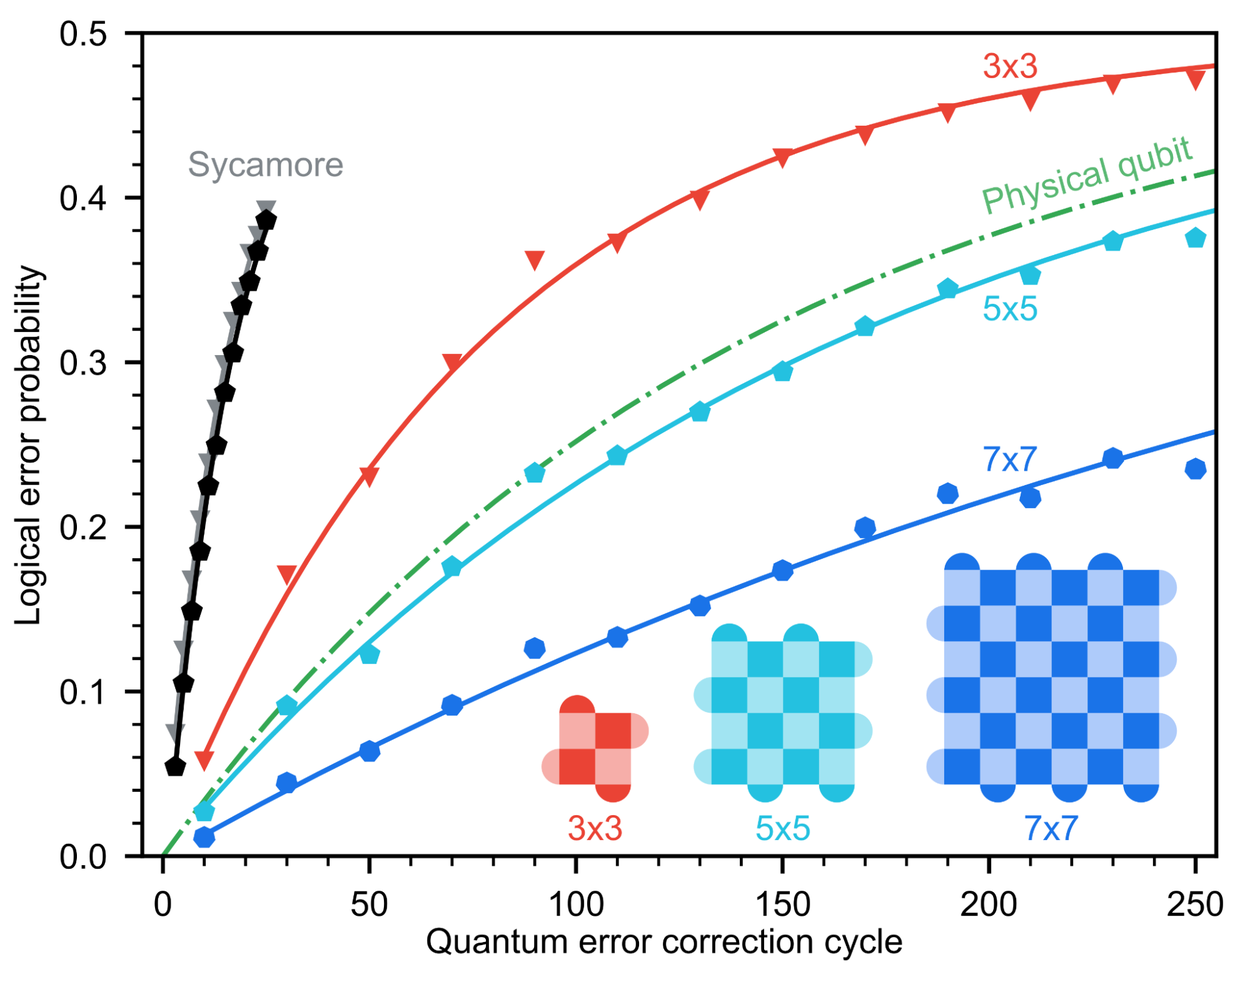
\includegraphics[width=0.7\linewidth]{img/Surface-Code-Scaling.png}
    \caption{Error Korrektur des 7x7 Surface Code \cite{acharya_quantum_2024}}
    \label{fig:Willow}
\end{figure}

Außerdem wurde durch die Anwendung des Surface Codes die $T_1$ Zeit von $20\mu s$ auf $68\mu s\pm13\mu s$ erhöht und ermöglich hierdurch mehr Operationen pro Qubit.\\